\documentclass[]{interact}

\graphicspath{{figures/}}

% Support for .eps illustrations
\usepackage{epstopdf}

% Support for small, `sub' figures and tables
\usepackage[caption=false]{subfig}

% To `separate' figures and tables from text if required
%\usepackage[nolists,tablesfirst]{endfloat}

% To produce a `double spaced' document if required
%\usepackage[doublespacing]{setspace}

% To increase paragraph indentation when line spacing is doubled
%\setlength\parindent{24pt}

% Citation support
\usepackage[natbibapa,nodoi]{apacite}
\setlength\bibhang{12pt}
\renewcommand\bibliographytypesize{\fontsize{10}{12}\selectfont}

% Theorem-like structures provided by amsthm.sty
\theoremstyle{plain}
\newtheorem{theorem}{Theorem}[section]
\newtheorem{lemma}[theorem]{Lemma}
\newtheorem{corollary}[theorem]{Corollary}
\newtheorem{proposition}[theorem]{Proposition}

\theoremstyle{definition}
\newtheorem{definition}[theorem]{Definition}
\newtheorem{example}[theorem]{Example}

\theoremstyle{remark}
\newtheorem{remark}{Remark}
\newtheorem{notation}{Notation}


%% Shorthand

\newcommand{\term}[1]{\emph{#1\/}}
\newcommand{\quotes}[1]{`#1'}

\newcommand{\comment}[2]
{
\begin{quote}
\textbf{#1:}
     #2
\end{quote}
}
%\renewcommand{\comment}[2]{}


\begin{document}

% Specify the article type or omit as appropriate
%\articletype{ARTICLE TEMPLATE}

\title{Reasoning}

\author{
  \name{Eirini Vandorou\textsuperscript{a,b}%
    \thanks{CONTACT E. Vandorou. Email: eirinivand@gmail.com}
    and Stasinos Konstantopoulos%
    \textsuperscript{b}}
  \affil{\textsuperscript{a}UniPi and NCSR? NCSR, while studying;
    \textsuperscript{b}Institute of Informatics and
    Telecommunications, NCSR \quotes{Demokritos}, Greece}
}
%% TODO: ask acharal and emiris if they want to contribute

\maketitle

\begin{abstract}
This articles is about reasoning.
\end{abstract}

\begin{keywords}
Reasoning; mathematics; Euclid
\end{keywords}


\section{Introduction}
\label{sec:intro}

\comment{TODO Stasinos}{later}


\section{Background}
\label{sec:bg}

\comment{TODO Discuss} {whether we could add that we are suggesting a way of 
assembling diagrams for custom and predefined proofs using the clojure library  
and some code. Possibly need to also address interactive proving.}

In this section we will go through some key characteristics about Euclid's 
Elements and relevant prior work. The current work can be summarized in the 
following sections; interactive theorem proving in geometry, automated 
deduction for geometry theorems \citep{avigad-etal:2009, beeson-etal:2019, 
miller:2001}, visualization of the theorem.

Although the Elements where considered flawless for many years,
Euclid's work was not as clear concerning the purity of logic.
Either that was because something came from observation or assumption, there
where many times in which Euclid would use non-logically proven
assumptions \citep[Sections~1.1 and~2]{harrison:2009}.
There have been some attempts to axiomatize, add to and fill the gaps of
Euclid's work. In this section we describe the latest approaches on refining
the Elements. However, we first need to understand a bit about Euclid's work
itself.

\subsection{The Elements}
The most widely known mathematician in geometry is Euclid form Ancient
Greece and Euclid's most renowned work are the \textit{Elements}
\citep{heath:1956}. The Elements consist of thirteen books, the first
six being about geometry of the plane and are based on the ruler-and-compass
approach. The first book contains five postulates and nine axioms along with
twenty three definitions and forty eight propositions. Postulates and axioms
may only be found in the first book. We based this work on the first book
because it contains the core elements that are used through out the Elements,
thus sets a solid base for implementing the rest as well.

Euclid’s propositions have a consistent structure; a set of statements, a
construction and a proof. The given statements are used to construct a diagram.
Then the proof is obtained using a combination of the given statements,
observations made on the diagram, definitions, postulates, axioms and
previously defined propositions.
\comment{Not sure if I should keep this possibly need to rephrase and/or add 
examples}{ The proofs are made specific enough to suit the needs of the
proposition, but also general enough to be applicable in different
situations. Which is made clear through out the Elements from the fact that
propositions are reapplied in many occasions. Occasions as such can be
propositions that even with a visually very different diagram, an earlier
proposition can be applied using a subset of the given statements or even
observations from the diagram of the current proposition.}
A basic characteristic of Euclid's
Elements is that each proposition once it is proven, it is considered
as given knowledge and so it is used inside other later propositions.


\subsection{Automated Deduction for Geometry Theorems}
\label{sec:atp-geometry}

The first to step in and axiomatize Euclid's work was \citet{hilbert:1899}.
He did this by redefining the basis of Euclid's definitions,
replacing and removing some axioms concerning the plane. There are
also other known axiomatizations of the Elements such as
\citet{tarski:1959} and \citet{birkhoff:1932}.

In recent years, \citet{avigad-etal:2009} presented a formal system that models
Books I to IV from Euclid's Elements. In order to address the matter
of facts that Euclid takes as observations from the diagram, they set
a list of axioms to replace them.

These axioms are in their core rules that depict
the diagram's purpose and part in the proof. They state that in some
cases where Euclid reads geometric relations directly from the
diagram, in their system this has to be met with one of the system's
rules. These axioms are divided into categories according to the
impact they depict from the diagram. The categories defined are the following.


\begin{list}{$\square$}{\leftmargin=3.5em \itemindent=0em}
	\item[\textit{construction rules}] These are the base of their axiom
	system and are described as the	\quotes{built-in theorems that are
	available from the start}. They include rules about
	points, lines, circles and intersections of the previous.

	\item[\textit{diagrammatic inference axioms}] These replace the diagram's
	purpose.
	 While traditional diagrammatic inference acts on manipulating a diagram,
	 this approach uses a set of axioms, construction and inference rules to
	 conclude on the \quotes{direct consequences} of those. They attempt to
	 define this notion and describe in which cases they work and why these
	 attempts may not be adequate.
	 \comment{TODO}{explain how these are not the same as diagrammatic 
	 inference below}
 
	 \item[\textit{transfer inference axioms}] Their intention is to depict how
	 the changes applied on a diagram by Euclid, translate to their facts.

	 \item[\textit{superposition inferences axioms}] these depict how one
	 diagram relates to another i.e. the rules that apply to the former apply
	 to the latter as well.
	 
	  \item[\textit{direct consequence}] They conclude this section by 
	  explaining the \quotes{direct consequence} notion, that they based their 
	  \quotes{diagrammatic inference} on. 
\end{list}


\begin{figure}[t]
  \centering
  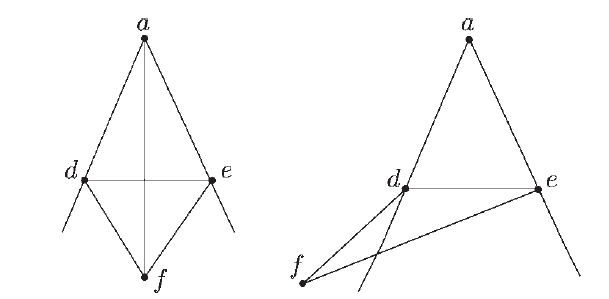
\includegraphics[scale=0.5]{avigad-fig8-I9}
  \caption[Avigad et al Approach I.9]{Two cases for Proposition~I.9
    considered by \citet{avigad-etal:2009}.}
  \label{fig:avigadi9}
\end{figure}


However, while Euclid takes
some parts of the construction as granted, in their system they claim
that more specificity is needed in order to make use of their rules.
One of the examples they give is Proposition I.9., where
Euclid generates a triangle $dfe$ (as seen in
Figure~\ref{fig:avigadi9}), they claim that the $f$ point needs more
clarification for its placing in the diagram because it may fall out
of the $dae$ angle, which is not true. If one follows Euclid's
direction for the construction the $f$ point does cut the angle in
half and it's impossible to be placed in the position they claim.
Euclid's directions state that to place the $f$ point one must
construct an equilateral triangle using his proposition I.1 with $de$
as a base. Creating an equilateral triangle would place point $f$
exactly in a positions precisely cutting the $dae$ angle in half when
one connects $f$ and $a$. Another example the use is the one of
proposition I.35 (as seen in Figure~\ref{fig:avigadi35}), in this case
there is a lot more to be discussed. While all three cases that they
present as figures can be generated solely from the proposition's
statement, the construction steps of the proposition eliminate the
second where there is one point less.

Euclid's aim is to prove the proposition, and while the proof
might not be exactly the same for all the cases considered in
Figure~\ref{fig:avigadi35}, the proposition is true for all which is
of most importance. Euclid is vague enough where he should be, since
his intend is to reuse the propositions through out his work, should
he have been more precise other proofs that use this one might not be
provable. It appears that Euclid is making use of the open world
assumption, which makes his work all the more attractive to potential
representation.

\begin{figure}[h]
  \centering
  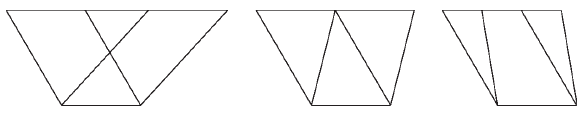
\includegraphics[scale=0.7]{avigad-fig9-I35}
  \caption[Avigad et al Approach I.35]{Three cases for
    Proposition~I.35 considered by Avigad et al. \cite{avigad-etal:2009}.}
  \label{fig:avigadi35}
\end{figure}


Last but not least, we will refer to their statement of Euclid not
stating enough information in his constructions. They take as an
example proposition I.2, claiming that point $a$ may not be inside
circle $\beta$ and a clarification of $da<dg$ should be made. This is
again misinterpreted since if one follows Euclid's steps to the
construction, even if $a$ fell out of circle the entire proof still
stands true. To prove this, one can consider the case where $ab>bc$
giving Figure~\ref{fig:prop-i2} (right). In this case the
circle with center $B$ (corresponding to circle $\alpha$ on the
left-hand side figure), would intersect with line
segment $Bd2$ (right) or $db$ (left) in two points.
\comment{TODO rewrite}{
When one takes the point that is between $d2$ and $B$ ($h2$) and
forms circle with center $d2$ and radius of $d2h2$ (right) or $\beta$ (left). 
Then line segment $Ad2$ intersects with the previous circle at point $l2$ and 
Euclid's proof stands exactly the same, even in this case, since again
the proposition's aim was to create a line segment from $A$ equal to
$BC$ and that is achieved.
}

\begin{figure}
  \centering

  \break
  \subfloat[Proposition~I.2 as formed by Avigad et al.]{%
    \resizebox*{0.4\textwidth}{!}{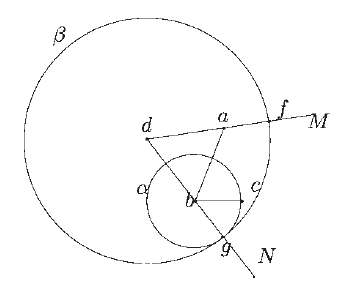
\includegraphics[scale=0.7]{avigad-I2}}}
  \hspace{3pt}
  \subfloat[The counter-example that Avigad et al. offer to argue that  ]{%
    \resizebox*{0.4\textwidth}{!}{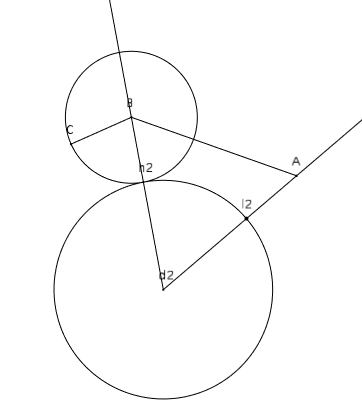
\includegraphics[scale=0.6]{avigad-I2-alt}}}
  \caption{Different diagrams that both support the proof of Proposition~I.2}
  \label{fig:prop-i2}
\end{figure}


The latest approach on Euclid
by \citet{beeson-etal:2019} approaches the matter of
\quotes{proof-checking Euclid}.
In their approach they used a custom-designed representation of
Euclid's Elements.

\comment{NOTE: Technical detail. To be deleted.}{
In this representation they merged every axiom, definition,
postulate, lemma and proposition into respective letters or
combination of such.  The most natural thing in doing so, following
Euclid, is to name variables with one character. Then, they used
two-character names for the relations since they exceed 24, and
used $AN$, $OR$ and $NO$ for conjuctions, disjunctions and
negations respectively. }

In their approach they do not follow Euclid's ways of proving and also
do not follow the same order as his. They seem to approach
superposition as equality between figures and define equality using 
\citet{hartshorne:2000} definitions redefined in first-order axioms.
What is more, they had to adapt to the tool and
reused theorems as implicit assumptions for each lemma.

\comment{TODO}{unclear. Explain how they solve or circumvent the 
core problem.}

They claim that their approach is more complete than previous
approaches to formalizing Euclid's work.  and that they are the first
to do a non-paper-and-pencil formalization.
They also claim that their work to add to Euclid's work and prove correct and 
valid Book I of Euclid, using their additions, including \quotes{corrected 
proofs of those propositions, that are close to Euclid's ideas}.


However, they too do not interpret superposition in the way Euclid
does and try to find other ways around this in the construction of
propositions and their proofs. For example, when they say that
proposition I.9 cannot be proved using I.1 and they try to work around
this.


\subsection{Diagrammatic Inference}
\label{sec:diagr-infer}

On the other hand, there are systems that act on diagrams like the one
of \citet{miller:2001}. In his approach Miller creates a
collection of rules that are divided into categories according to the
implication of the rule on the diagram, similar to the ones of Avigad
et al. First are the construction rules, inference rules follow and
then transformation rules. He treats superposition as
\term{lemma incorporation}, for which he defines and proves a theorem.
Miller's \term{Lemma Incorporation Theorem} is used in his system to
identify the forms that a diagram may take supposing an ancestor diagram.

\begin{figure}[t]
	\centering
	\subfloat[General representation of diagram from proposition I.1 ]{%
		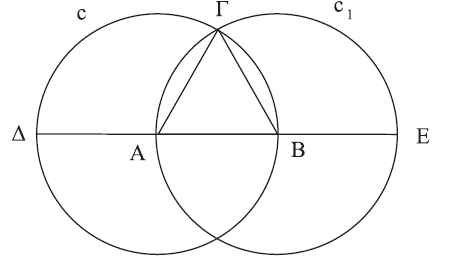
\includegraphics[width=\textwidth]{euclid-I1}}
	\hfil
	\subfloat[Resulting image of Proposition I.1 from \cite{miller:2001}. ]{%
		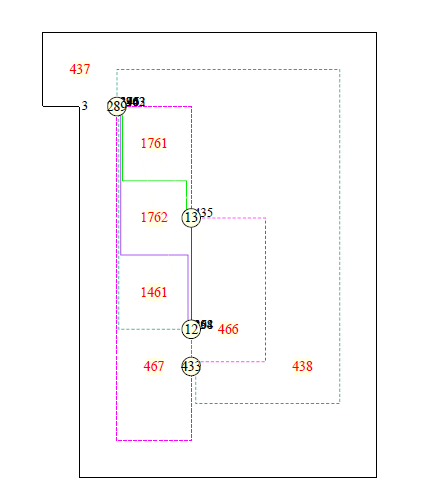
\includegraphics[width=\textwidth]{miller-fig320-I1}}
	
	\caption{Different representations of Proposition I.1}
	\label{fig:milleri1}
\end{figure}

This becomes useful in the sense of using this lemma to get the
superposition effect by isolating the diagram requiring superposition
from the parent diagram, applying is to a smaller \quotes{environment}
and using the result in the parent diagram. Miller concludes this
section with the presentation of the system CDEG that makes use of all
the above. CDEG diagrams are not as conservative and not easy to read,
an example diagram is the one of Figure~\ref{fig:milleri1} which is
the result of CDEG on proposition I.1 of Euclid.

The main issue with this approach is that it does not fully take
advantage of what Euclid essentially aims at, which is also the major
issue that most publications have difficulty interpreting.


\subsection{Remarks}

Euclid does indeed have some more vague points, on the contrary to
what these publications suggest, work best through his work, since the
vague points are not important to the application of a proposition,
rather opportunities to apply them even more times. The vague point
need no more clarification, if ones does specify in more detail the
context of each proposition might become more logically complete, but
it will lose the point of versatility.

One approach acts directly on diagrams
while others use solely logic to tackle the
problem. However, Euclid relies both on diagrams and logic in his
proofs. To encode so much information may be challenging, which means
that, isolating one or the other requires even more effort in
designing and applying such a method.



The notion of Functional Programming (FP) one would say is to
transform a problem into a set of steps one should 
execute, with the intent to focus on the computation of the problem.
Thus, instead of creating multiple paths for execution at a time,
functional programming focuses on one main goal and each function 
is a step towards this goal.

We aim that in this process, every step is a function, which 
itself is a part of the solution to a greater goal. A \textit{function} in 
FP takes a number of arguments, that it will use to compute the 
respective output. 



\section{We Need A Name}
\label{sec:foreground}

\comment{TODO Eirini}{later}


\section{Implementation and Validation}
\label{sec:impl}
\label{sec:eval}

\comment{TODO Eirini}{later}


\section{Conclusions}
\label{sec:conc}

\bibliographystyle{apacite}
\bibliography{references}

\end{document}
